\documentclass[10pt]{article}
\usepackage[spanish]{babel}
\selectlanguage{spanish}
\usepackage[utf8]{inputenc}
\usepackage{graphicx}
\usepackage[lmargin=3cm,rmargin=3cm,tmargin=3cm,bmargin=3cm]{geometry}
\usepackage{amsmath}
\usepackage{amsfonts}
\usepackage{amssymb}
\title{Mareas}
\author{Luisa Fernanda Orci Fernandez.}
\date{08 de Mayo del 2015}


\begin{document}

\maketitle

\section{Marea}
Es el cambio periódico del nivel del mar, producido por la fuerza de atracción gravitatoria que ejercen la luna y el sol sobre el Planeta Tierra. \\

Desde la antigüedad se conoce este fenómeno, pero fue Isaac Newtown en el año de 1687 con su obra "Principios matemáticos de la Filosofía Natural", quien dio la explicación de las mareas, la cual es aceptada hoy en día. 

\section{Un poco de teoría}
La teoría de las mareas es cuando aplicamos la mecánica de medios continuos para predecir e interpretar la deformacion de cuerpos planetarios y satélites, así como la de sus atmósferas y océanos, a partir de la carga gravitacional de otro cuerpo como la luna sobre la tierra. \\


En 1775 Pierre-Simon Laplace describió la reacción del océano a las fuerzas de la marea. La teoría de Laplace tomó en cuenta la resonancia, los períodos naturales de las cuencas oceánicas, así como la fricción. 

\newpage

\section{Programa en FORTRAN}


Este programa de FORTRAN fue diseñado para encontrar las  mareas máximas y mínimas de cada mes, así como su periodo.

\subsection{Código en FORTRAN}
\begin{verbatim}
program Mareas

implicit none

real, dimension (7674) :: altura

integer :: i 

real :: Datos1, MaxDia1, MaxDia2, MaxDia3
real :: Maxima1, Maxima2, Maxima3, Maxima4, Maxima5
real :: Tiempo11, Tiempo12, Tiempo13, Tiempo14, Tiempo15
real :: Datos2, MinDia1, MinDia2, MinDia3
real :: Minima1, Minima2, Minima3, Minima4, Minima5
real :: Tiempo21, Tiempo22, Tiempo23, Tiempo24, Tiempo25
real :: Tiempox1, Tiempox2, Tiempox3
real :: Tiempon1, Tiempon2, Tiempon3
real :: PeriodoMesMax1, PeriodoMesMax2, PeriodoMesMax3, PeriodoMesMax4
real :: PeriodoMesMax5
real :: PeriodoMesMin1, PeriodoMesMin2, PeriodoMesMin3, PeriodoMesMin4
real :: PeriodoMesMin5
real :: PeriodoDiaMax1, PeriodoDiaMax2, PeriodoDiaMax3
real :: PeriodoDiaMin1, PeriodoDiaMin2, PeriodoDiaMin3
real :: PeriodoMesMaximo
real :: PeriodoMesMinimo
real :: PeriodoDiaMaximo
real :: PeriodoDiaMinimo



open (1, file = "Mareas.csv")

do i = 1, 7674
read (1, *) altura(i)
end do
close (1)

! MES UNO

Maxima1 = 0
do i = 1, 1344
Datos1 = Maxima1 - altura(i)
if (Datos1<0) then 
Maxima1 = altura(i)

Tiempo11 = i/48.0
end if
end do

Minima1 = 0
do i = 1, 1344
Datos2 = Minima1 - Altura(i)
if (Datos2>0) then
Minima1 = altura(i)

Tiempo21 = i/48.0
end if
end do

!MES DOS

Maxima2 = 0
do i = 1345, 2689
Datos1 = Maxima2 - altura(i)
if (Datos1<0) then 
Maxima2 = Altura(i)

Tiempo12 = i/48.0
end if 
end do

Minima2 = 0
do i = 1345, 2689
Datos2 = Minima2 - altura(i)
if (Datos2>0) then
Minima2 = altura(i)

Tiempo22 = i/48.0
end if
end do

!MES TRES

Maxima3 = 0
do i = 2690, 4034
Datos1 = Maxima3 - altura(i)
if (Datos1<0) then
Maxima3 = altura(i)

Tiempo13 = i/48.0
end if
end do

Minima3 = 0
do i = 2690, 4034
Datos2 = Minima3 - altura(i)
if (Datos2>0) then
Minima3 = altura(i)

Tiempo23 = i/48.0
end if
end do


!MES CUATRO

Maxima4 = 0
do i = 4035, 5379
Datos1 = Maxima4 - altura(i)
if (Datos1<0) then
Maxima4 = altura(i)

Tiempo14 = i/48.0
end if
end do

Minima4 = 0
do i = 4035, 5379
Datos2 = Minima4 - altura(i)
if (Datos2>0) then
Minima4 = altura(i)

Tiempo24 = i/48.0
end if
end do

!MES CINCO

Maxima5 = 0
do i = 5380, 6724
Datos1 = Maxima5 - altura(i)
if (Datos1<0) then
Maxima5 = altura(i)

Tiempo15 = i/48.0
end if
end do

Minima5 = 0
do i = 5380, 6724
Datos2 = Minima5 - altura(i)
if (Datos2>0) then
Minima5 = altura(i)

Tiempo25 = i/48.0
end if
end do 

! --------------------------

MaxDia1 = 0 
do i = 1, 48
Datos1 = MaxDia1 - altura(i)
if(Datos1<0) then 
MaxDia1 = altura(i)

Tiempox1 = i * 0.5

end if 
end do

MinDia1 = 0
do i = 1, 48
Datos2 = MinDia1 - altura(i)
if (Datos2>0) then
MinDia1 = altura(i)

Tiempon1 = i * 0.5

end if
end do

! --------------------------

MaxDia2 = 0
do i = 49, 97
Datos1 = MaxDia2 - altura(i)
if (Datos2<0) then
MaxDia2 = altura(i)

Tiempox2 = i * 0.5

end if
end do

MinDia2 = 0 
do i = 49, 97
Datos2 = MinDia2 - altura(i)
if (Datos2>0) then
MinDia2 = altura(i)

Tiempon2 = i * 0.5

end if 
end do

! ----------------------------

MaxDia3 = 0
do i = 98, 146
Datos1 = MaxDia3 - altura(i)
if (Datos1<0) then
MaxDia3 = altura(i)

Tiempox3 = i * 0.5

end if
end do

MinDia3 = 0
do i = 98, 146
Datos2 = MinDia3 - altura(i)
if (Datos2>0) then 
MinDia3 = altura(i)

Tiempon3 = i * 0.5

end if 
end do 

! PERIODOS

PeriodoMesMax1 = Tiempo11
PeriodoMesMax2 = Tiempo12 - Tiempo11
PeriodoMesMax3 = Tiempo13 - Tiempo12
PeriodoMesMax4 = Tiempo14 - Tiempo13
PeriodoMesMax5 = Tiempo15 - Tiempo14

PeriodoMesMin1 = Tiempo21
PeriodoMesMin2 = Tiempo22 - Tiempo21
PeriodoMesMin3 = Tiempo23 - Tiempo22
PeriodoMesMin4 = Tiempo24 - Tiempo23
PeriodoMesMin5 = Tiempo25 - Tiempo24

PeriodoDiaMax1 = Tiempox1
PeriodoDiaMax2 = Tiempox2 - Tiempox1
PeriodoDiaMax3 = Tiempox3 - Tiempox2

PeriodoDiaMin1 = Tiempon1
PeriodoDiaMin2 = Tiempon2 - Tiempon1
PeriodoDiaMin3 = Tiempon3 - Tiempon2

! PERIODOS MAXIMOS Y MINIMOS

PeriodoMesMaximo = ( PeriodoMesMax1 + 
PeriodoMesMax2 + PeriodoMesMax3 + PeriodoMesMax4 + PeriodoMesMax5 ) / 5.0
PeriodoMesMinimo = ( PeriodoMesMin1 + 
PeriodoMesMin2 + PeriodoMesMin3 + PeriodoMesMin4 + PeriodoMesMin5 ) / 5.0

PeriodoDiaMaximo = ( PeriodoDiaMax1 + PeriodoDiaMax2 + PeriodoDiaMax3 ) / 3.0
PeriodoDiaMinimo = ( PeriodoDiaMin1 + PeriodoDiaMin2 + PeriodoDiaMin3 ) / 3.0





Print * , ' ========================================================== '
Print * , 'ALTURA MAXIMA DE LAS MAREA'
Print * , ' ========================================================== '
Print * , 'Día 1:' , MaxDia1
Print * , 'Día 2:' , MaxDia2
Print * , 'Día 3:' , MaxDia3
Print * , ' ========================================================== '
Print * , 'Mes uno:' , Maxima1 , 'En el día:' , Tiempo11
Print * , 'Mes dos:' , Maxima2 , 'En el día:' , Tiempo12
Print * , 'Mes tres:' , Maxima3 , 'En el día:' , Tiempo13
Print * , 'Mes cuatro:' , Maxima4 , 'En el día:' , Tiempo14
Print * , 'Mes cinco:' , Maxima5 , 'En el día:' , Tiempo15
Print * , ' ========================================================== '
Print * , 'ALTURA MINIMA DE LA MAREA'
Print * , ' ========================================================== '
Print * , 'Día 1:' , MinDia1
Print * , 'Día 2:' , MinDia2
Print * , 'Día 3:' , MinDia3
Print * , ' ========================================================== '
Print * , 'Mes uno:' , Minima1 , 'En el día:' , Tiempo21
Print * , 'Mes dos:' , Minima2 , 'En el día:' , Tiempo22
Print * , 'Mes tres:' , Minima3 , 'En el día:' , Tiempo23
Print * , 'Mes cuatro:' , Minima4 , 'En el día:' , Tiempo24
Print * , 'Mes cinco:' , Minima5 , 'En el día:' , Tiempo25
Print * , ' ========================================================== '
Print * , ' PERIODO MAXIMO POR MES '
Print * , ' ========================================================== '
Print * , 'Periodo 1:' , PeriodoMesMax1
Print * , 'Periodo 2:' , PeriodoMesMax2
Print * , 'Periodo 3:' , PeriodoMesMax3
Print * , 'Periodo 4:' , PeriodoMesMax4
Print * , 'Periodo 5:' , PeriodoMesMax5
Print * , ' ========================================================== '
Print * , 'PERIODO MINIMO POR MES'
Print * , ' ========================================================== '
Print * , 'Periodo 1:' , PeriodoMesMin1
Print * , 'Periodo 2:' , PeriodoMesMin2
Print * , 'Periodo 3:' , PeriodoMesMin3
Print * , 'Periodo 4:' , PeriodoMesMin4
Print * , 'Periodo 5:' , PeriodoMesMin5
Print * , ' ========================================================== '
Print * , ' PERIODO MAXIMO POR DIA '
Print * , ' ========================================================== '
Print * , 'Periodo 1:' , PeriodoDiaMax1
Print * , 'Periodo 2:' , PeriodoDiaMax2
Print * , 'Periodo 3:' , PeriodoDiaMax3
Print * , ' ========================================================== '
Print * , ' PERIODO MINIMO POR DIA '
Print * , ' ========================================================== '
Print * , 'Periodo 1:' , PeriodoDiaMin1
Print * , 'Periodo 2:' , PeriodoDiaMin2
Print * , 'Periodo 3:' , PeriodoDiaMin3
Print * , ' ========================================================== '
Print * , 'PROMEDIO DEL PERIODO MAXIMO Y MINIMO POR MES:' 
Print * , 'Maximo:' , PeriodoMesMaximo
Print * , 'Minimo:' , PeriodoMesMinimo
Print * , ' ========================================================== '
Print * , 'PROMEDIO DEL PERIODO MAXIMO Y MINIMO POR DIA:'
Print * , 'Maximo:' , PeriodoDiaMaximo
Print * , 'Minimo:' , PeriodoDiaMinimo

 


end program Mareas

\end{verbatim}


\newpage
\subsection{Resultados en pantalla}

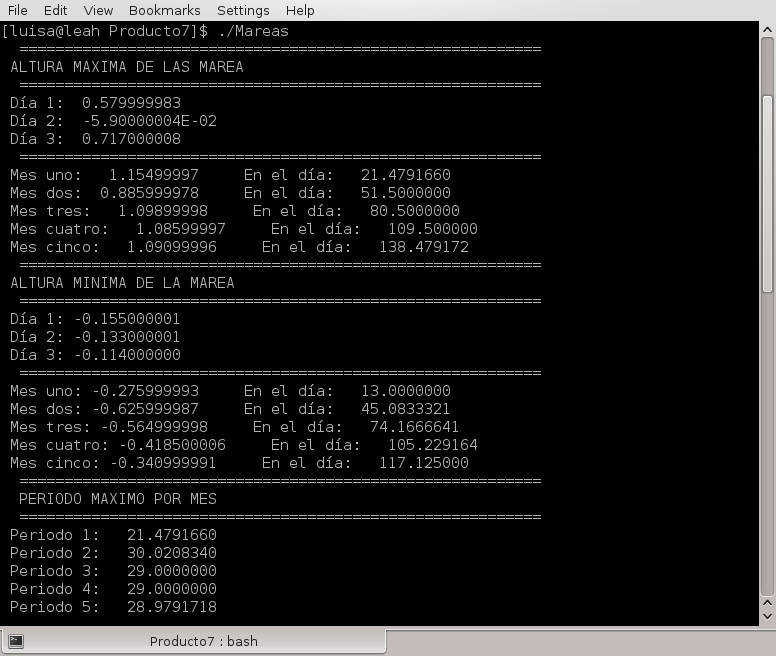
\includegraphics[scale=0.6]{resultadomarea1.png} \\ 
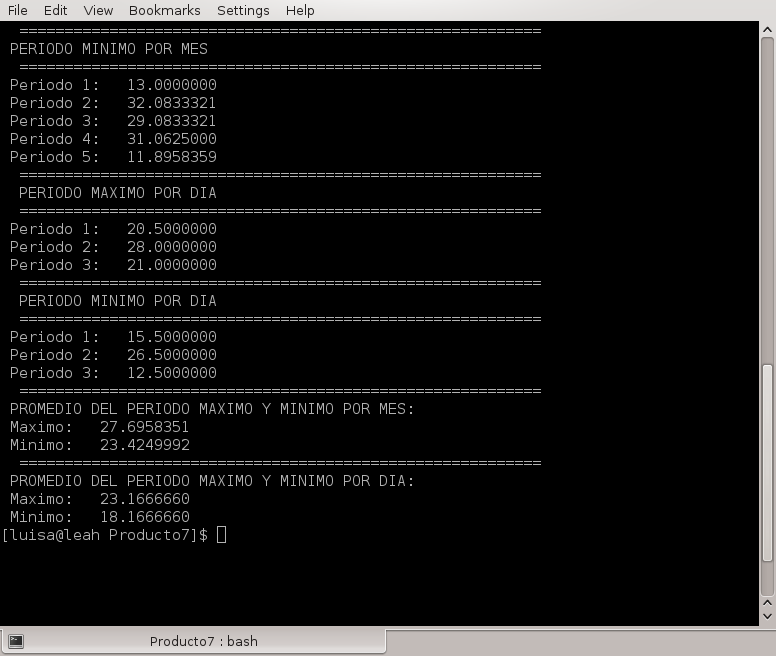
\includegraphics[scale=0.6]{resultadomarea2.png}

\newpage

\subsection{Gráficas}
A continuación, las gráficas de los máximos y mínimos por mes y por días de las mareas. 

\subsubsection{Gráfica de todos los meses}
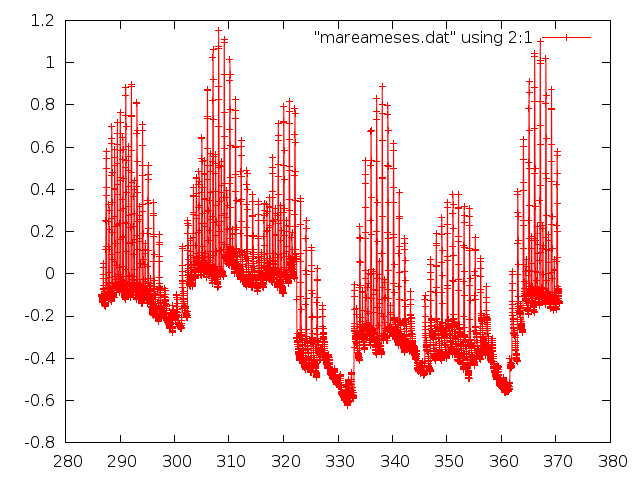
\includegraphics[scale=0.6]{mareameses.png}

\subsubsection{Mes 1}
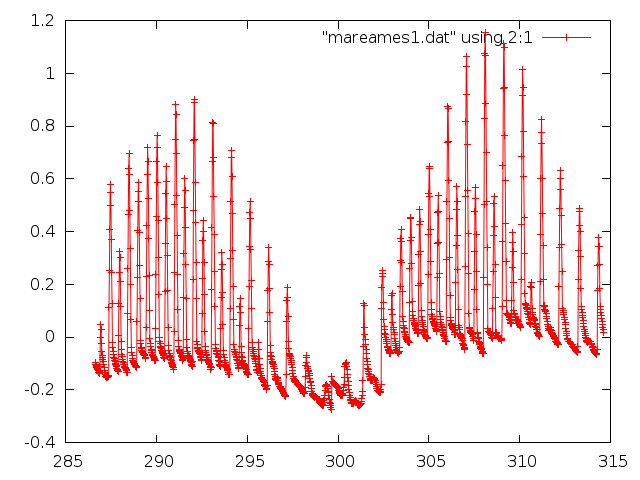
\includegraphics[scale=0.6]{mareames1.png}

\subsubsection{Mes 2}
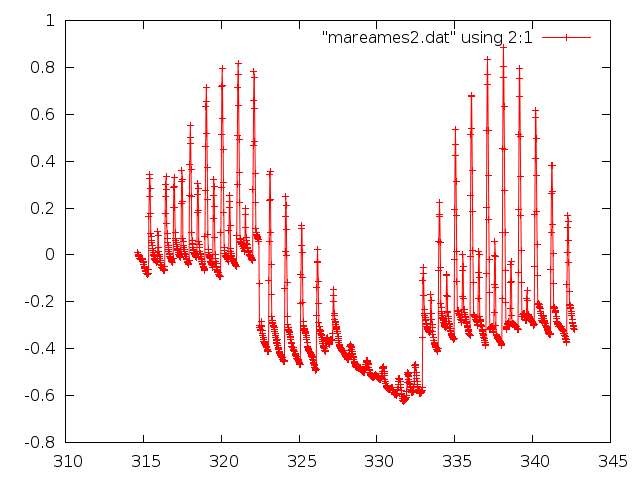
\includegraphics[scale=0.6]{mareames2.png}

\subsubsection{Mes 3}
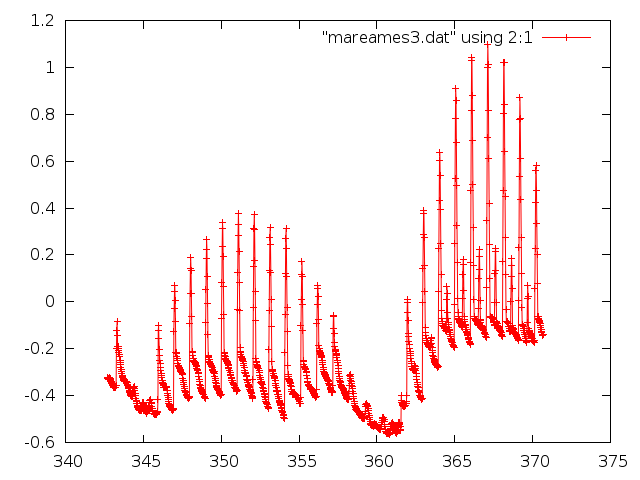
\includegraphics[scale=0.6]{mareames3.png}

\newpage

\subsubsection{Gráfica de todos los días}
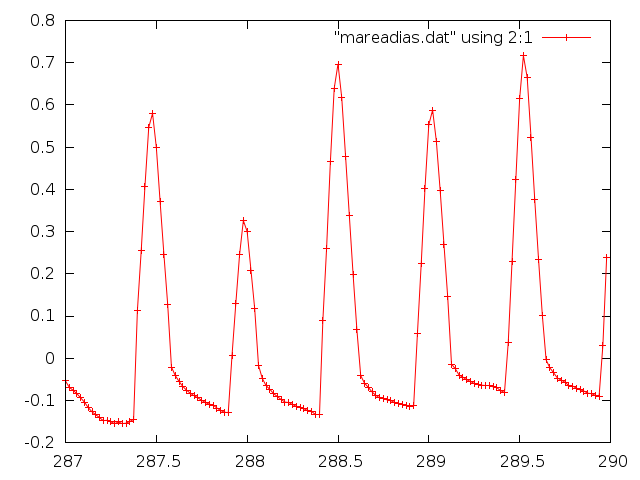
\includegraphics[scale=0.6]{mareadias.png}

\subsubsection{Día 1}
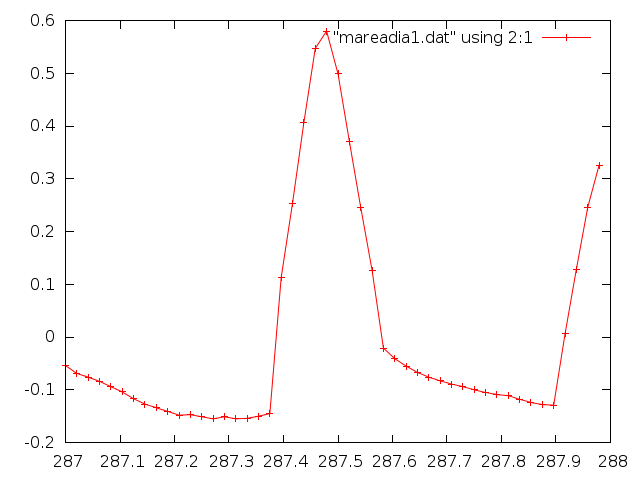
\includegraphics[scale=0.6]{mareadia1.png}

\subsubsection{Día 2}
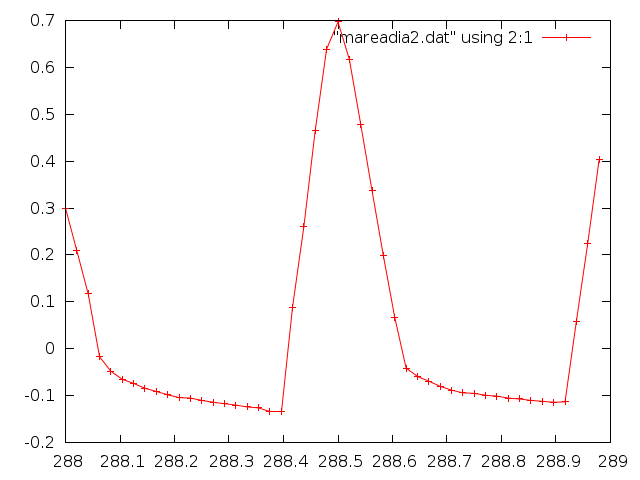
\includegraphics[scale=0.6]{mareadia2.png}

\subsubsection{Día 3}
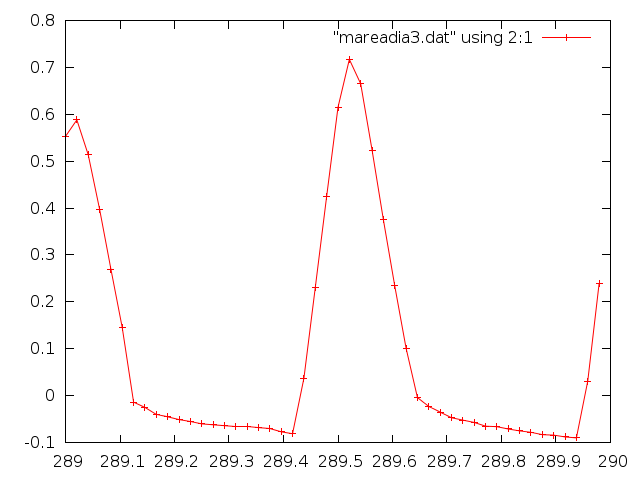
\includegraphics[scale=0.6]{mareadia3.png}





\end{document}